%%% tfs_core.tex --- 
%%
%% Author: yzf<yzf@net.pku.edu.cn>
%% Version: $Id: tfs_core.tex,v 0.0 2007/06/14 02:40:55 yzf Exp$
%% Note: use pdfLaTeX

%\revision$Header: /home/yzf/tmp/tfs_core.tex,v 0.0 2007/06/14 02:40:55 yzf Exp$
\documentclass[11pt,a4paper]{scrartcl}
\usepackage{CJKutf8}
\usepackage{indentfirst}
\usepackage[debugshow,final]{graphics}
\addtolength{\hoffset}{-0.5cm}
\addtolength{\textwidth}{1cm}
\bibliographystyle{acm} % plain,abbrv,alpha,apalike,unsrt,acm,ieeetr,siam
\usepackage{url}
%\frenchspacing
%\pagestyle{headings}
\usepackage[pdftex,bookmarks,colorlinks,linkcolor=red,citecolor=green,filecolor=magenta,urlcolor=blue,unicode]{hyperref}

%%================================================================
%% begin document
%%================================================================
\begin{document}
\begin{CJK*}{UTF8}{gbsn}
\CJKcaption{zh-Hans}
\title{TFS文件操作的语义和流程 \protect\footnote{I $\heartsuit$ \LaTeX{} and GNU Emacs :)}}
\author{\CJKfamily{gkai}\href{http://net.pku.edu.cn/~yzf/}{杨志丰}$<$\href{mailto:yzf@net.pku.edu.cn}{yzf@net.pku.edu.cn}$>$}
\date{\today}
\maketitle
%\tableofcontents

\section*{前言}
在我们的设计过程中,多次讨论过TFS文件系统中核心文件操作的语义(用户层面
的,以及master-client,master-chunkserver通讯层面的)。本文档的目的是整
理我们的思路和明确我们最终的决定,重点在于强调我们的不同之处。

首先,回顾GFS论文中对read, write, append(即atomic record append)等操
作的语义的说明。然后,总结一下hadoop实现中这些操作时的语义。最后,结合
我们设计,回顾我们思路的转变过程,明确最终决定选用的语义。
\section{GFS中文件操作的语义}
\subsection{文件块}
对于系统中的所有块大小是固定的,为64M。每一个块都有一个版本号,master
端记录当前每个块的最新版本号,当它发现chunkserver报告的块的版本号小于最新
版本号时,说明该chunkserver在这个块被更新时恰好系统出错,master可以
指示chunkserver删除这个复本。
\subsection{读}
首先,使用固定的块大小,client把offset转换为文件中的块序号。
然后,他把文件名和块序号发送给master,master返回对应的块标识和存储
位置。client缓存这些信息,client选择一个最近的包含该块的
chunkserver,发送块标识和块内的一块字节区域请求chunkserver发送数据。
client端缓存的元数据在一定时间之后失效。

\subsection{写}
在已有文件内任意位置的写操作是允许的,但是这种操作不保证高效。
使用租约(lease)机制来保证对一个块的多个复本修改操作的执行顺序
(见~\cite{gfs2003}~3.1节)。并发的写操作是允许的,但是结果是不确定的(很可能
含有多个写操作的片段),但是只要写成功,租约保证了多个复本内容是一致的。

\subsection{记录追加写}
系统高效的支持多个client同时对同一个文件进行追加操作。
记录追加写使用和写操作同样的租约机制。在操作成功个区域内,数据是在
各个复本上是一致,并且数据是完整的,但是在不成功的区域中数据在各个
复本上是不一致的。所以,记录可能有重复,并且可能有系统填充的空白。

\subsection{应用程序的约定}
应用程序最好通过追加而不是改写来修
改数据;应用程序在文件中设置检查点(checkpoint),并且包含应用一级
自己的数据校验和,因为并发的写操作可能产生错误的数据。使用记录追加
写的应用,要在记录中包含校验和,从而在使用时发现填充的空白和不完整
的记录。记录追加写可能产生重复的记录,应用可以通过在记录中包含唯一
的标识符来剔除重复的记录。
\subsection{锁}
名字空间的每一个结点(文件或目录)都有一个锁。根据操作的不同性质,
要给涉及操作的所有结点上读锁或写锁。为了避免死锁,上锁的顺序必须一
致。
\section{Hadoop中文件操作的语义}
本部分参考hadoop-0.8.0的代码~\cite{hadoop},以及一篇介绍hadoop体系结构的文档~\cite{hadooparch}。

\subsection{文件块}
每个文件可以在创建时指定它的最大块的大小。块大小是可变的,所以
它是块的属性之一(此外,还有ID)。

\subsection{应用模型}
文件被创建并且一次写完,关闭之后就不能修改(将来计划加入追加
写的操作)。Hadoop的这种文件访问模式被叫做write-once-read-many。
自然的,Hadoop不支持多写者的原子的记录追加写。
\subsection{读}
\label{sec:hadoopread}
应用程序(准确的说,是文件系统的客户端库,下同)通过一个输入流读取
文件的数据。当他打开文件的输入流的时候,
从master得到所有属于这个文件的所有块的标识,以及每一个块的存储位置。因为文件
创建之后是不可以修改的,所以它的会信息是不变的,这种一次性的通讯策略因此
正确而高效。进而,客户端可以根据得到的所有块的长度信息算出文件长度。这之后,
读取指定字节区域的数据就是很自然可以想到的过程了。
\subsection{写}
因为Hadoop中,文件只能写一次,所以文件的创建过程就是写文件数据的过程。
一般的文件都很大,为了提高性能,hadoop使用了“两级”缓存机制,写入的数据首
先缓存在内存中,这个缓存的大小默认为4K字节,可以通过系统属性io.file.buffer.size定制。
当数据超出内存缓存大小的时候,把它写入本地的一个缓冲文件中。当文件的大小等于
文件定义的块大小的时候,应用程序向master申请一个新的块,然后把整个块写入master
指定的chunkserver上。

具体的数据传输过程如下:应用程序和master返回的多个chunkserver中的第一个
建立连接。如果连接失败,则重试若干次。如果重试都失败,并且当且要写入的块是
文件的第一个块,则通知master放弃整个文件(namenode.abandonFileInProgress);
如果当前要写入的不是第一块,则通知master放弃这个块的写入(namenode.abandonBlock)。
如果连接成功,应用程序把数据以及其他要保存块的复本chunkserver信息传给第一个chunkserver,
第一个chunkserver把数据保存在本地的同时,又把它同时传给下一个chunkserver(以此类推)。
如果第一个chunkserver的本地文件写失败了(比如,因为磁盘空间不够),那么它通知应用程序这次写
失败了。({\color{red}实际上不是通过直接用返回值或异常来通知应用端。chunkserver端发现写错误
后直接关闭与client通讯的socket连接,
client的底层库读不到应有的回应,就认为写出错。因为client和chunkserver的通讯使用了简单
的客户服务器socket通讯,而没有使用可靠的RPC机制,所以这样做也可以发现通讯失败造成的错误。
})应用程序可以选择重试写,或者放弃。如果第一个
chunkserver的本地写成功了,
然后它会收集还有哪些chunkserver成功的接收了数据,把成功接收数据的所有chunkserver(至少有1个)报告给应用程序。
应用程序再把这个信息报告给master(namenode.reportWrittenBlock(locatedchunk)),然后继续后序的写操作。
master接收到这个信息,把他们记录在他的核心元数据中(chunk--chunkserver映射,chunkserver--chunks映射)。
所以,一个块写成功\emph{当且仅当}第一个chunkserver写成功,而不管其他chunkserver是否
写成功。

与读数据一样,应用程序写数据也是通过一个输出流实现的。这个输出流能(并且只能)创建文件操作之后得到。Master要
记录每一个正在被创建的文件,不允许一个正在被创建的文件被多次创建(当然,一个已经创建好的文件
允许被覆盖,相当于删除后新建一个文件),所以,同一个文件不允许被同时写。
\section{TFS文件操作语义}
Hadoop要求一个文件从创建时开始写一直到结束,为了支持这种操作,master
中增加了createPending等信息保留创建过程中的信息。这就需要master维护客
户端的很多状态信息。另一个局限是,文件在创建之后就不能修改了。我们的系
统希望能支持GFS论文中支持的基本操作:支持高效的并发的读取;支持随机的写操作,
但不必高效;支持高效的并发的原子的追加操作。GFS中为了支持他定义的一致
性模型,修改操作(包括写和原子追加)都需要比较复杂的租约机制来支持。我
们在设计中试图不使用租约,而通过其他方法避免复杂性。同时,
设计时紧紧围绕两个“尽量”:尽量
减少client和master之间的通讯;尽量减少master维护的客户端信息。
\subsection{文件块}
文件块大小是可变的,所以块的大小是块的一个属性。每一个块都有一个版本号,master
端记录当前每个块的最新版本号,当它发现chunkserver报告的块的版本号小于最新
版本号时,说明该chunkserver在这个块被更新时恰好系统出错,master可以
指示chunkserver删除这个复本。所以,版本号也是块的一个属性。
\subsection{应用模型}
把创建操作和写操作严格区分开来。客户端要新建一个文件,只是在master的名
字空间中添加一个项。一个新文件被创建之后,它的大小为0。随后,应用程序
可以可以通过追加操作来写数据。追加操
作是可并发的。应用程序也可以通过普通写操作来改写已经存在的文件块。这种
随机写操作是不可以并发的。注意,本节内容所说的“追加”特指系统提供的一个文
件操作,而不包括用“从文件末尾开始写起”的“普通”写操作。
\subsection{读}
应用程序通过以只读方式打开一个文件,打开文件的同时从master得到所有属于
这个文件的块的信息。同时,master会把相应的文件上读锁,防止文件在读的过
程中被其他应用程序删除,也防止文件在被读的同时被其他应用程序修改。
{\color{red}一个文件被打开后,如果其它用户删除了这个文件,
那么一般的语义是:free-on-last-close,
即当最后一个访问者关闭文件结束访问时,系统会删除这个文件。}

通讯的基本操作参见\ref{sec:hadoopread}。
\subsection{写}\label{subsec:tfswrite}
应用程序以写方式打开一个文件之后,master会把相应的文件上排他锁,不允许
其他应用程序同时写它,也不允许读或追加。有两种可能的情况,下面分别讨论。

如果应用程序要写的字节区域位于已有的块上,则程序得到块的存储位置后,把
数据传给第一个chunkserver,第一个chunkserver把修改写到本地的同时把数据
传给下一个chunkserver,以此类推,形成一个数据流水线。修改成功({\color{red}为了保证
数据确实写入了本地永久存储,chunk-server要使用本地文件系统的fsync()来
把缓存和磁盘同步})使得块复本
的版本号加一。流水线的下一级都向上一级报告它的后续流水线上每个
chunkserver修改操作成功与否(除了通信错误,最可能的出错原因是磁盘空间
不够),并附带自己的。这样,
第一个chunkserver就知道所有chunkserver成功与否的信息(如果流水线的一级中通信出
错,也没有关系),只要至少有一个成功了,就向应用报告成功,并把成功的
chunkserver报告给应用程序,应用程序在把他通过
ClientService.completeWrittenChunk报告给master。master由此
把块的最新版本号加一,并更新他的核心元数据(chunk--chunkserver映射,
chunkserver--chunks映射)。那些没有被更新的块复本会在将来的垃圾回收时
被清理掉。如果第一个chunkserver发现没有一个修改成功,
则向应用程序报告写失败,应用程序可以根据失败原因选择重试或者放弃。(参见图~\ref{fig:write})

这里之所以不使用像hadoop那样的策略,即只要第一个chunkserver失败就认为
操作失败,是因为对于修改已有块的修改操作,如果非第一个chunkserver成功
了,这种修改是不能被撤销也不能被忽视的。{\color{red}(比如,图~\ref{fig:write}中
cs1和cs2写失败,而cs3写成功了的情况下,我们应该认为本次操作成功了。否则,
cs3上复本的修改master不知道,系统认为块没有被修改,版本号不增加。这样的块在当前
使用版本号来发现无效块的机制中是无法被发现的
)而hadoop的策略对于仅支持块的添
加操作是足够的,因为新块没有被系统记录在系统元数据前,即使在物理上存在,将来也可以
被垃圾回收的。所以,我们的“写操作失败”的语义是,所有的块复本都失败了。}
\begin{figure}
  \centering
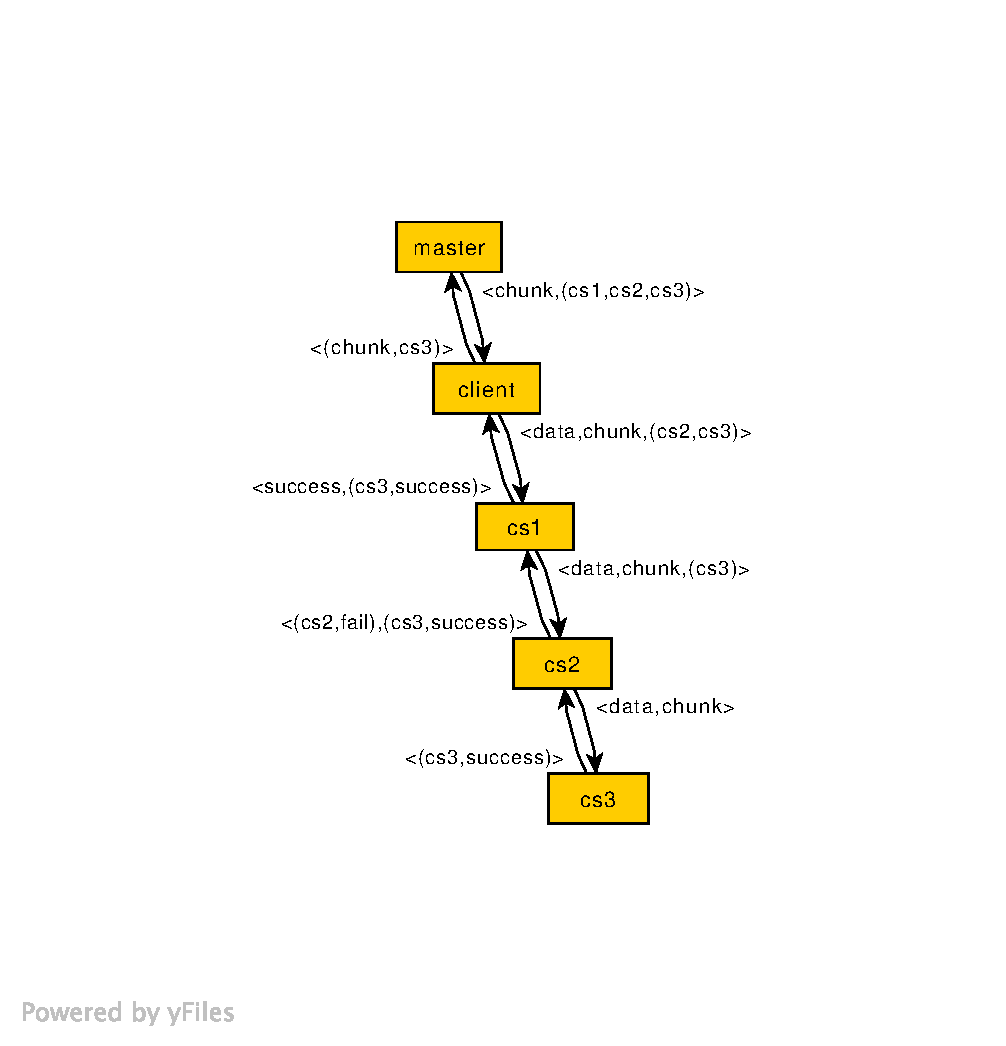
\includegraphics{tfswrite}  
  \caption{流水化写操作}
  \label{fig:write}
\end{figure}

如果应用程序要写的区域超出当前文件长度({\color{red}即一般意义上的append操作,也就是
应用指定的写入位置为文件末尾。注意,如果应用指定的写入位置超出文件长度,系统
返回错误}),则应用程序通过
ClientService.addChunk
向master申请一个新的
块。master会记录当前正在被新建的块。后续的操作同前面所述类似。如果写成
功,应用程序通过ClientService.complete-AddChunk把写成功的块以及写成功的
复本所在chunkserver信息报告给master。master可以由此更新他的核心元数据。
如果写失败,一般情况下,应用可以选择重试,重新分配一个块。当然,在此之
前,应用要通过ClientService.abandonAddChunk把失败报告给master。
master可以删除记录的数据。
\subsection{记录追加写}
我们的追加写和GFS的追加写是不同的。因为块大小可变,所以系统不会
自动在文件中添充空白。我们的追加写是以块为单位的写,所以它是
exactly-once,而不是at-least-once,一次追加
操作不会产生重复的数据。他是可以并发的,多个应用程序可以并发的对一个文
件追加数据,但是系统不保证并发写入的不同块之间的顺序。

应用程序以追加方式打开一个文件之后,master会把相应的文件上读锁,防止文
件被删除,但同时其他应用程序可以读取它,也可以追加。

追加操作的其他语义和~\ref{subsec:tfswrite}小节中“应用程序要写的区域
超出当前文件长度”的情况一样。应用程序调用追加操作时,只提供数据,而不
用指定写入位置,并且,数据的大小必须小于这个文件的块大小({\color{red}为了保证数据的
完整性。因为系统只能保证文件块的完整性,大于块大小的数据系统不知道如何分割
才能保证其内部记录格式的完整})。底层client向
master申请一个新的块,然后写入。所以,每次
追加操作无论数据多少都会产生新的块,这就要求应用程序尽量以长度恰好为块
大小或接近块大小调用追加操作。否则,之后读取的效率可能“异常”的低。

{\color{red}
追加操作是原子的,每一个追加操作保证数据的完整性。但系统不保证多个
append操作之间的顺序与数据存储顺序一致,即,应用程序的两次连续的追加操
作,最终可能产生的文件块(在读取文件时)在逻辑上并不相邻。

为了优化性能,append不是Synchronous操作,而采用dealy-write。即当
append()调用结束,系统并不保证数据已经保存在永久存储里了,而是写入
cache后立刻返回,系统在之后的某个时间,把cache数据写到chunkserver上去。
这样带来的另一个好处是,系统有可能对多个追加操作产生的小块进行合并,合
并之后再写到chunkserver上去。delay-write缺点是:极端情况下,追加写的
数据会丢失。错误无法在调用时发现。如果应用程序想要保证数据永久存储,可
以使用系统在client库提供fsync()操作来执行数据同步和错误检查。
}
\subsection{应用程序约定}
对于能表示为某种记录格式的数据,应用程序最好通过记录追加写而不是普通写来添加
数据;{\color{red}使用记录追加写的应用,如果可以接受delay-write可能产生的错误,最好
不使用系统提供的fsync。}应用程序的两次连续的追加操作,最终可能产生的文件
块(在读取文件时)在逻辑上并不相邻。
\bibliography{myBib} % my bibliography database
\end{CJK*}
\end{document}

%%% Local Variables: 
%%% mode: latex
%%% coding: utf-8
%%% TeX-master: t
%%% End: 
